\documentclass[dvipsnames,tikz]{standalone}
\usepackage{amsmath}
\usepackage{arevmath}
\usepackage{xcolor}
\usepackage{tikz}
\usetikzlibrary{calc}
\usetikzlibrary{decorations.pathreplacing,calligraphy,3d}

\tikzset{main/.style={draw=white, circle, color=white}}
\tikzset{main_gray/.style={draw=white, circle, color=white, opacity=0.1}}
%change to gray!20 for light style

\begin{document}
		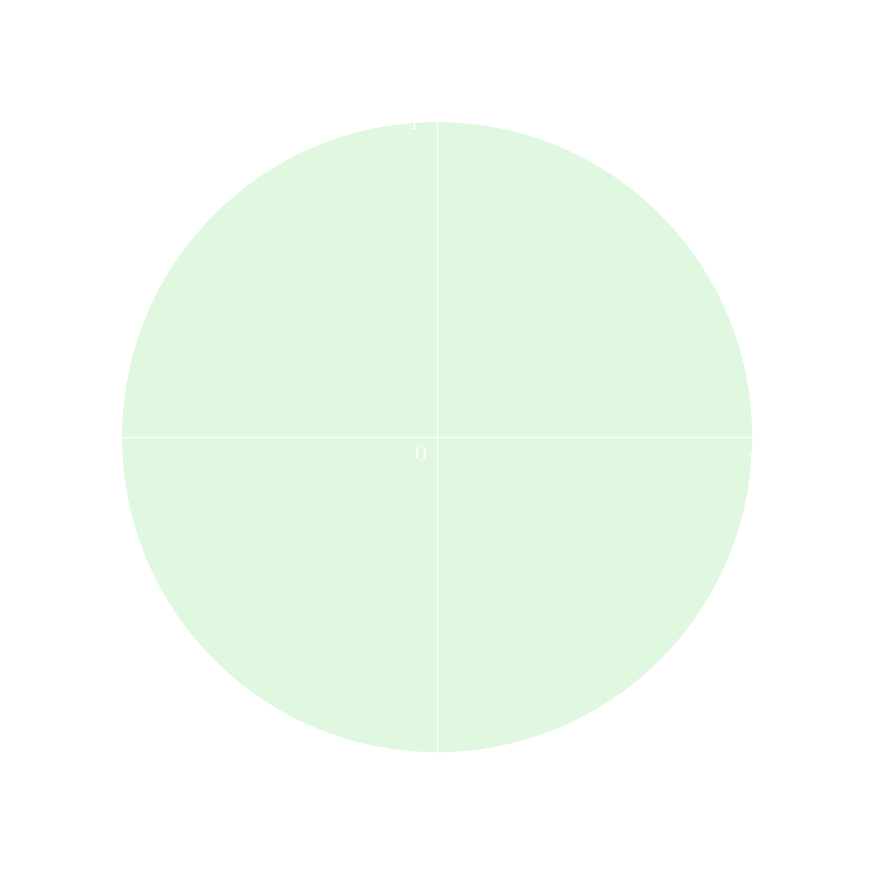
\begin{tikzpicture}[scale=1, main, line join=bevel, font=\small]
			\clip (-5.2,-5.2) rectangle (5.2,5.2);
			\draw[step=0.4, main_gray]  (-5.2,-5.2) grid (5.2,5.2);
			\draw[main, dashed] (-4,-4) rectangle (4,4);
			\fill[fill=LimeGreen, fill opacity=0.15] (0,0) circle (4cm);
			\draw[main] (0,0) node [below left] {\footnotesize $0$};
			\draw[main] (4,0) node [below] {\footnotesize $1$};
			\draw[main] (0,4) node [left] {\footnotesize $1$};
			\draw[main, -stealth] (-5,0) -- (5,0) node [below] {$x$};
			\draw[main, -stealth] (0,-5) -- (0,5) node [left] {$y$};
		\end{tikzpicture}
	
		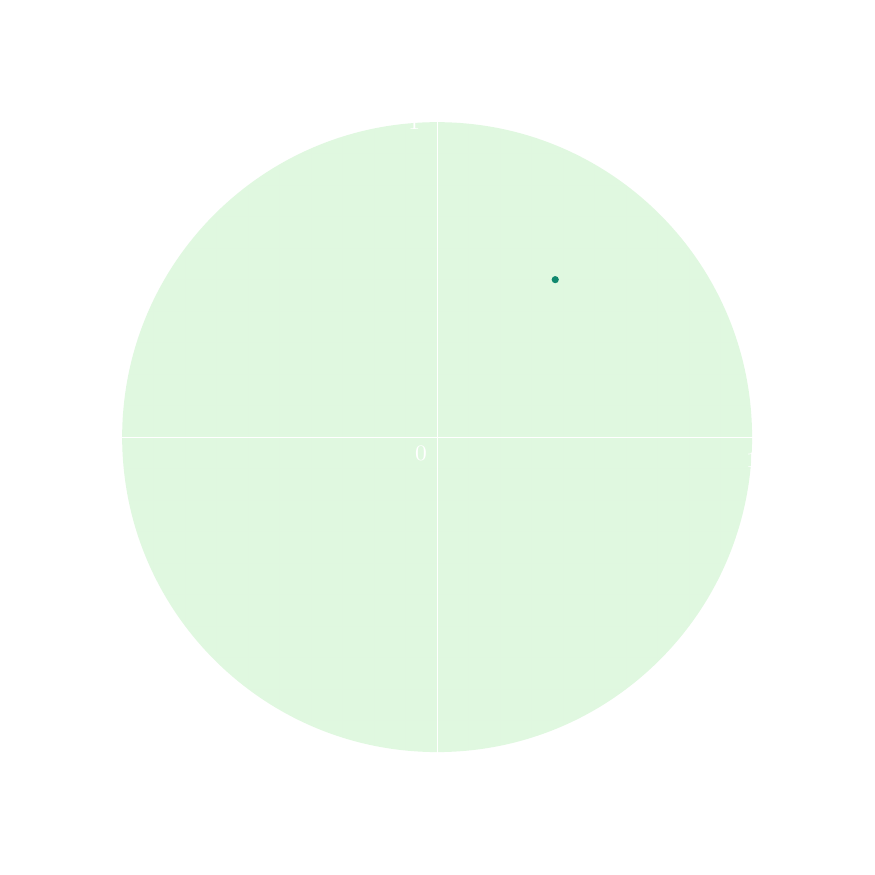
\begin{tikzpicture}[scale=1, main, line join=bevel, font=\small]
			\clip (-5.2,-5.2) rectangle (5.2,5.2);
			\draw[step=0.4, main_gray]  (-5.2,-5.2) grid (5.2,5.2);
			\draw[main, dashed] (-4,-4) rectangle (4,4);
			\fill[fill=LimeGreen, fill opacity=0.15] (0,0) circle (4cm);
			\draw[main] (0,0) node [below left] {\footnotesize $0$};
			\draw[main] (4,0) node [below] {\footnotesize $1$};
			\draw[main] (0,4) node [left] {\footnotesize $1$};
			\draw[main, -stealth] (-5,0) -- (5,0) node [below] {$x$};
			\draw[main, -stealth] (0,-5) -- (0,5) node [left] {$y$};
			
			\fill [PineGreen] (1.5,2) circle (1.3pt);
		\end{tikzpicture}
		
		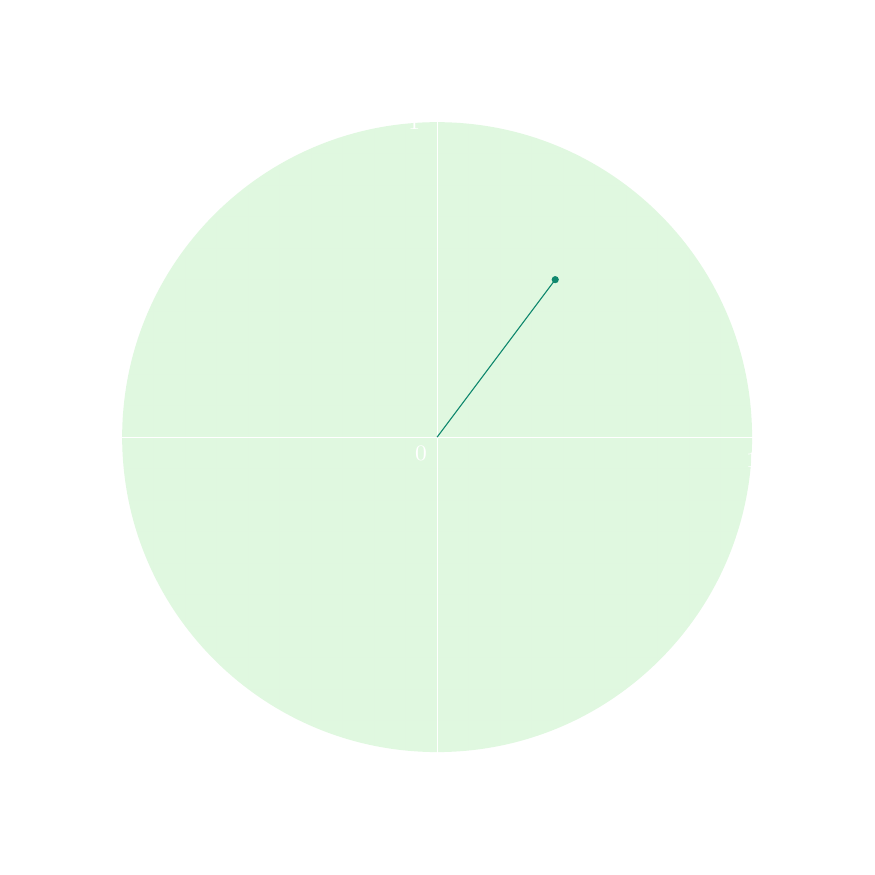
\begin{tikzpicture}[scale=1, main, line join=bevel, font=\small]
			\clip (-5.2,-5.2) rectangle (5.2,5.2);
			\draw[step=0.4, main_gray]  (-5.2,-5.2) grid (5.2,5.2);
			\draw[main, dashed] (-4,-4) rectangle (4,4);
			\fill[fill=LimeGreen, fill opacity=0.15] (0,0) circle (4cm);
			\draw[main] (0,0) node [below left] {\footnotesize $0$};
			\draw[main] (4,0) node [below] {\footnotesize $1$};
			\draw[main] (0,4) node [left] {\footnotesize $1$};
			\draw[-stealth] (-5,0) -- (5,0) node [below] {$x$};
			\draw[-stealth] (0,-5) -- (0,5) node [left] {$y$};
			
			\fill [PineGreen] (1.5,2) circle (1.3pt);
			\draw [PineGreen] (0,0) -- (1.5,2);
		\end{tikzpicture}
		
		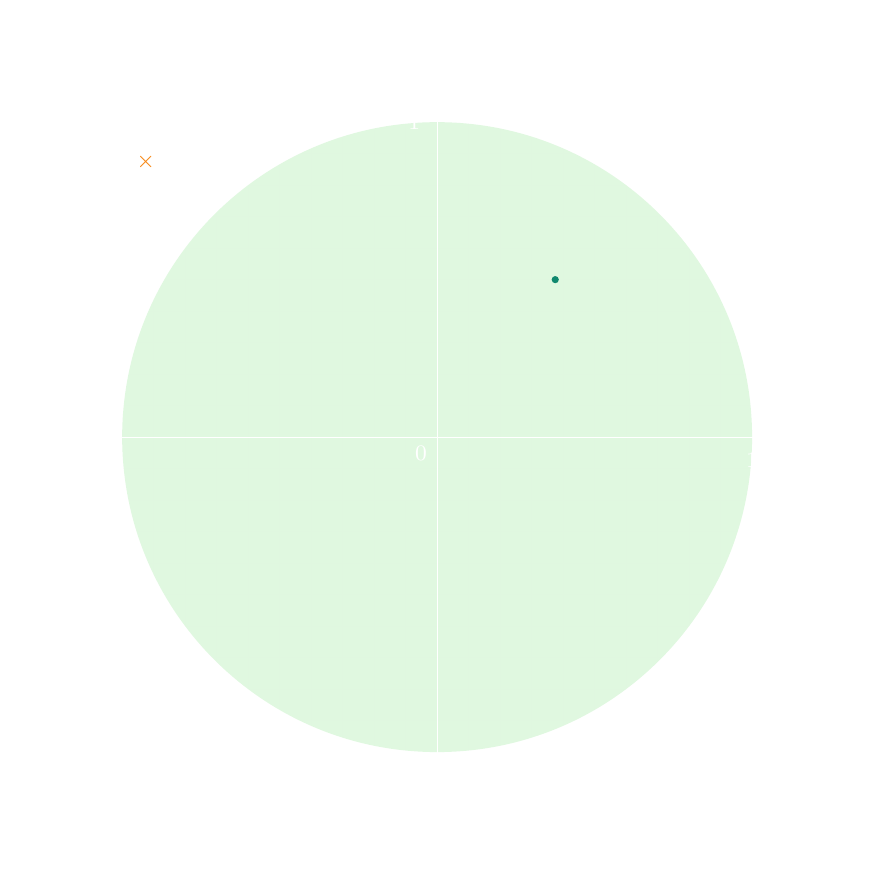
\begin{tikzpicture}[scale=1, main, line join=bevel, font=\small]
			\clip (-5.2,-5.2) rectangle (5.2,5.2);
			\draw[step=0.4, main_gray]  (-5.2,-5.2) grid (5.2,5.2);
			\draw[main, dashed] (-4,-4) rectangle (4,4);
			\fill[fill=LimeGreen, fill opacity=0.15] (0,0) circle (4cm);
			\draw[main] (0,0) node [below left] {\footnotesize $0$};
			\draw[main] (4,0) node [below] {\footnotesize $1$};
			\draw[main] (0,4) node [left] {\footnotesize $1$};
			\draw[main, -stealth] (-5,0) -- (5,0) node [below] {$x$};
			\draw[main, -stealth] (0,-5) -- (0,5) node [left] {$y$};
			
			\fill [color=PineGreen] (1.5,2) circle (1.3pt);
			\draw [color=BurntOrange,](-3.7,3.5) node {\footnotesize $\times$};
		\end{tikzpicture}
		
		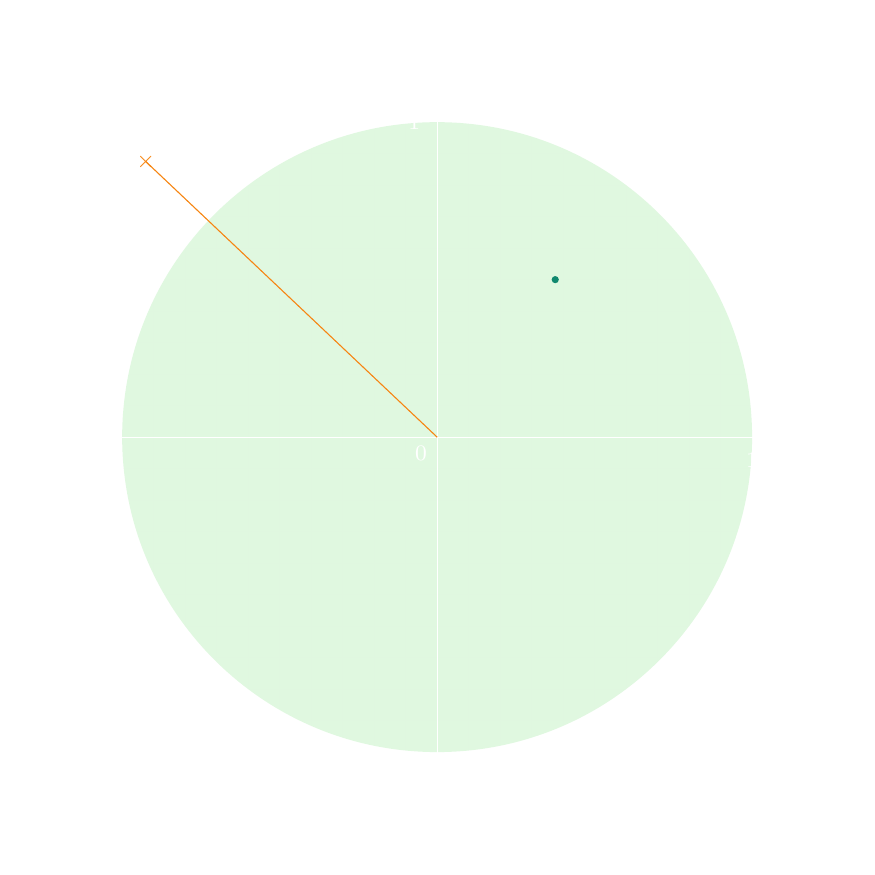
\begin{tikzpicture}[scale=1, main, line join=bevel, font=\small]
			\clip (-5.2,-5.2) rectangle (5.2,5.2);
			\draw[step=0.4, main_gray]  (-5.2,-5.2) grid (5.2,5.2);
			\draw[main, dashed] (-4,-4) rectangle (4,4);
			\fill[fill=LimeGreen, fill opacity=0.15] (0,0) circle (4cm);
			\draw (0,0) node [below left] {\footnotesize $0$};
			\draw (4,0) node [below] {\footnotesize $1$};
			\draw (0,4) node [left] {\footnotesize $1$};
			\draw[main, -stealth] (-5,0) -- (5,0) node [below] {$x$};
			\draw[main, -stealth] (0,-5) -- (0,5) node [left] {$y$};
			
			\fill [PineGreen] (1.5,2) circle (1.3pt);
			\draw [BurntOrange,](-3.7,3.5) node {\footnotesize $\times$};
			\draw [BurntOrange] (0,0) -- (-3.7,3.5);
		\end{tikzpicture}
		
		\pgfmathsetseed{123}
		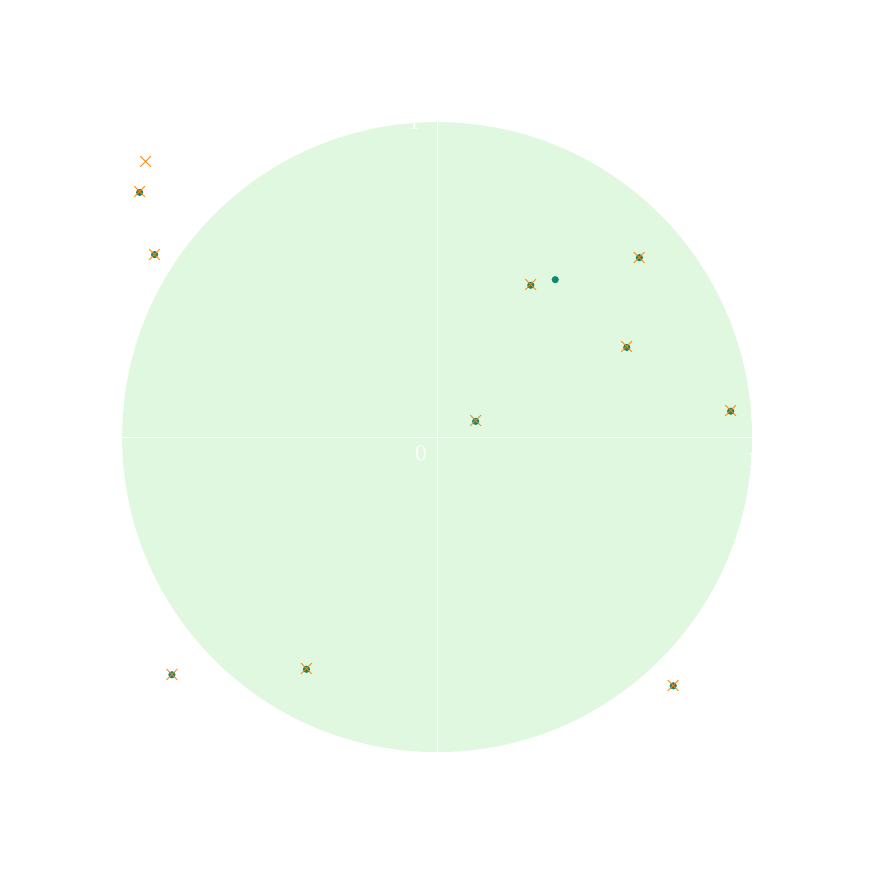
\begin{tikzpicture}[scale=1, main, line join=bevel, font=\small]
			\clip (-5.2,-5.2) rectangle (5.2,5.2);
			\draw[step=0.4, main_gray]  (-5.2,-5.2) grid (5.2,5.2);
			\draw[main, dashed] (-4,-4) rectangle (4,4);
			\fill[fill=LimeGreen, fill opacity=0.15] (0,0) circle (4cm);
			\draw[main] (0,0) node [below left] {\footnotesize $0$};
			\draw[main] (4,0) node [below] {\footnotesize $1$};
			\draw[main] (0,4) node [left] {\footnotesize $1$};
			\draw[main, -stealth] (-5,0) -- (5,0) node [below] {$x$};
			\draw[main, -stealth] (0,-5) -- (0,5) node [left] {$y$};
			
			\fill [PineGreen] (1.5,2) circle (1.3pt);
			\draw [BurntOrange,](-3.7,3.5) node {\footnotesize $\times$};
			
			\foreach \i in {1,...,10} {
				\pgfmathrandominteger{\a}{-400}{400}
				\pgfmathrandominteger{\b}{-400}{400}
				\pgfmathparse{less(sqrt(\a*0.01*\a*0.01 + \b*0.01*\b*0.01),4)}
				\let\c\pgfmathresult
				
				\ifthenelse{\c = 1}{
					\fill [color=PineGreen](\a*0.01,\b*0.01) circle (1.3pt);
				}{
					\draw [color=BurntOrange,](\a*0.01,\b*0.01) node {\footnotesize $\times$};
				}
			}
		\end{tikzpicture}
		
		\pgfmathsetseed{123}
		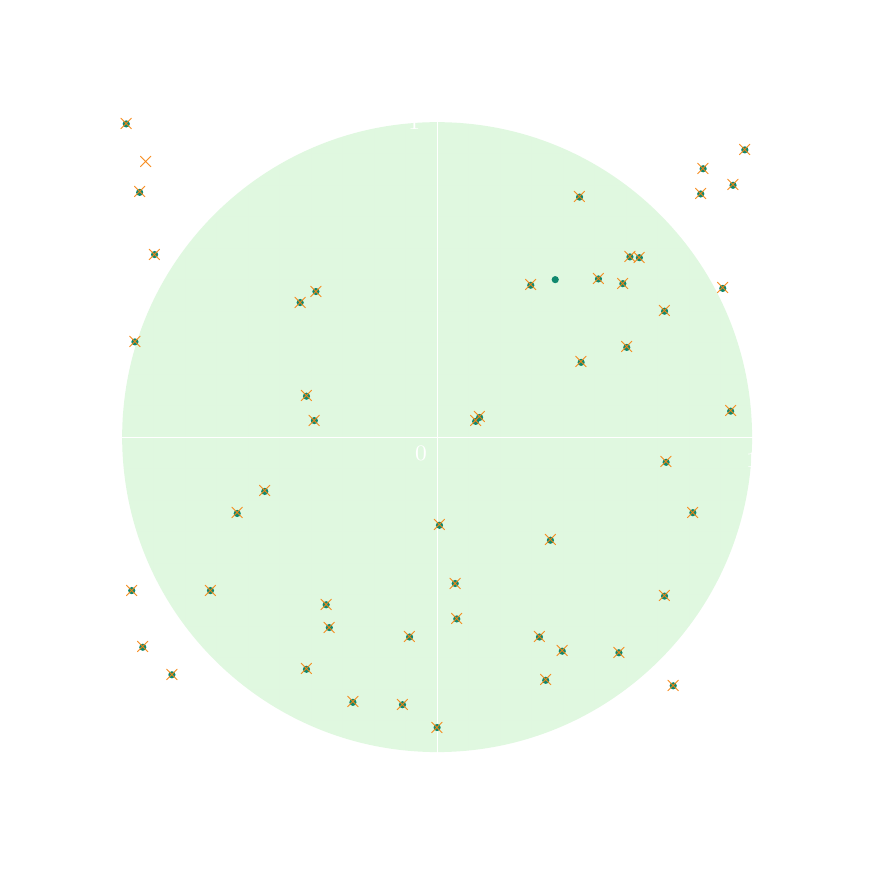
\begin{tikzpicture}[scale=1, main, line join=bevel, font=\small]
			\clip (-5.2,-5.2) rectangle (5.2,5.2);
			\draw[step=0.4, main_gray]  (-5.2,-5.2) grid (5.2,5.2);
			\draw[main, dashed] (-4,-4) rectangle (4,4);
			\fill[fill=LimeGreen, fill opacity=0.15] (0,0) circle (4cm);
			\draw[main] (0,0) node [below left] {\footnotesize $0$};
			\draw[main] (4,0) node [below] {\footnotesize $1$};
			\draw[main] (0,4) node [left] {\footnotesize $1$};
			\draw[main, -stealth] (-5,0) -- (5,0) node [below] {$x$};
			\draw[main, -stealth] (0,-5) -- (0,5) node [left] {$y$};
			
			\fill [PineGreen] (1.5,2) circle (1.3pt);
			\draw [BurntOrange,](-3.7,3.5) node {\footnotesize $\times$};
			
			\foreach \i in {1,...,50} {
				\pgfmathrandominteger{\a}{-400}{400}
				\pgfmathrandominteger{\b}{-400}{400}
				\pgfmathparse{less(sqrt(\a*0.01*\a*0.01 + \b*0.01*\b*0.01),4)}
				\let\c\pgfmathresult
				
				\ifthenelse{\c = 1}{
					\fill [color=PineGreen](\a*0.01,\b*0.01) circle (1.3pt);
				}{
					\draw [color=BurntOrange,](\a*0.01,\b*0.01) node {\footnotesize $\times$};
				}
			}
		\end{tikzpicture}
		
		\pgfmathsetseed{123}
		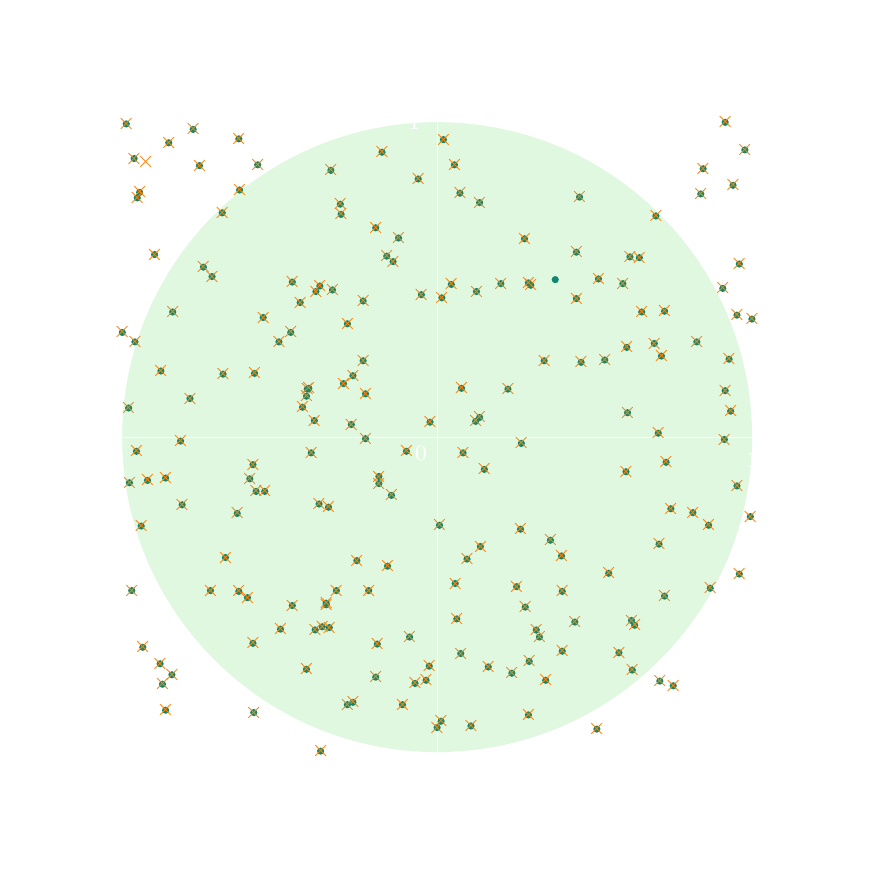
\begin{tikzpicture}[scale=1, main, line join=bevel, font=\small]
			\clip (-5.2,-5.2) rectangle (5.2,5.2);
			\draw[step=0.4, main_gray]  (-5.2,-5.2) grid (5.2,5.2);
			\draw[main, dashed] (-4,-4) rectangle (4,4);
			\fill[fill=LimeGreen, fill opacity=0.15] (0,0) circle (4cm);
			\draw[main] (0,0) node [below left] {\footnotesize $0$};
			\draw[main] (4,0) node [below] {\footnotesize $1$};
			\draw[main] (0,4) node [left] {\footnotesize $1$};
			\draw[main, -stealth] (-5,0) -- (5,0) node [below] {$x$};
			\draw[main, -stealth] (0,-5) -- (0,5) node [left] {$y$};
			
			\fill [PineGreen] (1.5,2) circle (1.3pt);
			\draw [BurntOrange,](-3.7,3.5) node {\footnotesize $\times$};
			
			\foreach \i in {1,...,200} {
				\pgfmathrandominteger{\a}{-400}{400}
				\pgfmathrandominteger{\b}{-400}{400}
				\pgfmathparse{less(sqrt(\a*0.01*\a*0.01 + \b*0.01*\b*0.01),4)}
				\let\c\pgfmathresult
				
				\ifthenelse{\c = 1}{
					\fill [color=PineGreen](\a*0.01,\b*0.01) circle (1.3pt);
				}{
					\draw [color=BurntOrange,](\a*0.01,\b*0.01) node {\footnotesize $\times$};
				}
			}
		\end{tikzpicture}
		
		\pgfmathsetseed{123}
		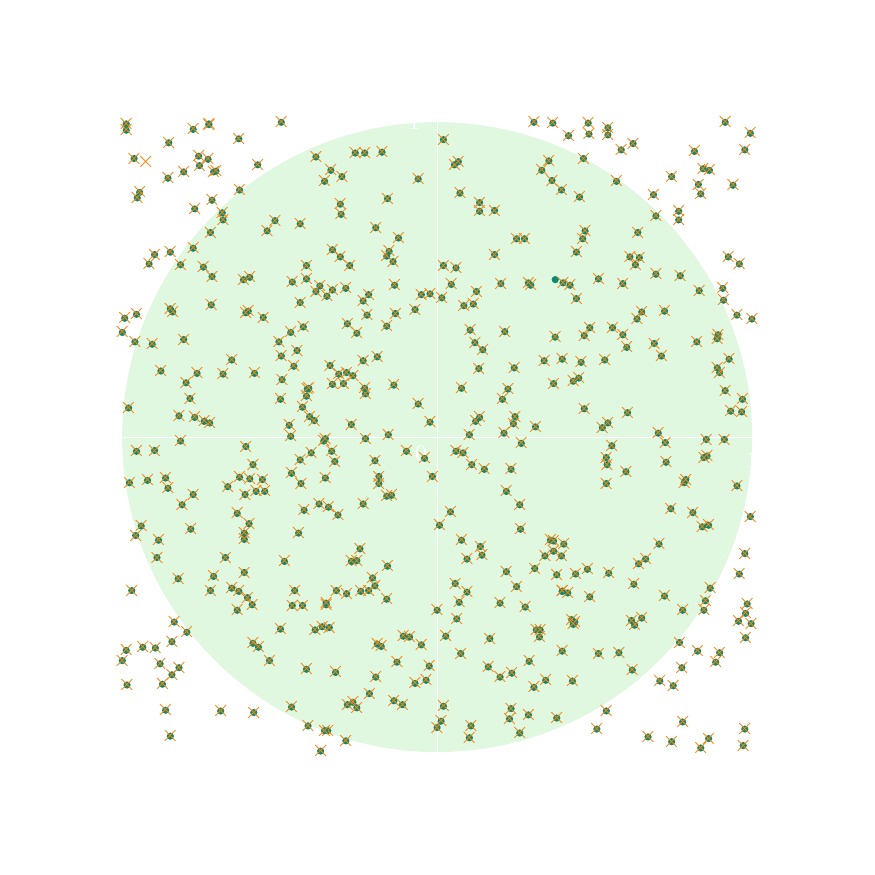
\begin{tikzpicture}[scale=1, main, line join=bevel, font=\small]
			\clip (-5.2,-5.2) rectangle (5.2,5.2);
			\draw[step=0.4, main_gray]  (-5.2,-5.2) grid (5.2,5.2);
			\draw[main, dashed] (-4,-4) rectangle (4,4);
			\fill[fill=LimeGreen, fill opacity=0.15] (0,0) circle (4cm);
			\draw[main] (0,0) node [below left] {\footnotesize $0$};
			\draw[main] (4,0) node [below] {\footnotesize $1$};
			\draw[main] (0,4) node [left] {\footnotesize $1$};
			\draw[main, -stealth] (-5,0) -- (5,0) node [below] {$x$};
			\draw[main, -stealth] (0,-5) -- (0,5) node [left] {$y$};
			
			\fill [PineGreen] (1.5,2) circle (1.3pt);
			\draw [BurntOrange,](-3.7,3.5) node {\footnotesize $\times$};
			
			\foreach \i in {1,...,500} {
				\pgfmathrandominteger{\a}{-400}{400}
				\pgfmathrandominteger{\b}{-400}{400}
				\pgfmathparse{less(sqrt(\a*0.01*\a*0.01 + \b*0.01*\b*0.01),4)}
				\let\c\pgfmathresult
				
				\ifthenelse{\c = 1}{
					\fill [color=PineGreen](\a*0.01,\b*0.01) circle (1.3pt);
				}{
					\draw [color=BurntOrange,](\a*0.01,\b*0.01) node {\footnotesize $\times$};
				}
			}
		\end{tikzpicture}
\end{document}